\documentclass[10pt, a4paper]{article}
\usepackage[top=3cm, bottom=4cm, left=3.5cm, right=3.5cm]{geometry}
\usepackage{amsmath,amsthm,amsfonts,amssymb,amscd, fancyhdr, color, comment, graphicx, environ}
\usepackage{float}
\usepackage{mathtools}
\usepackage{mathrsfs}
\usepackage[math-style=ISO]{unicode-math}
\DeclareSymbolFont{\mathnormal}{letters}
\usepackage{lastpage}

%%%%%%%%%%%%%%%%%%%%%%%%%%%%%%%%%%%%%%%%%%%%%%%%%%%%%%%%%%%%%%%%%%
%%%%%%%%%%%%%%%%%%%%%%%%%%%%%%%%%%%%%%%%%%%%%%%%%%%%%%%%%%%%%%%%%%
%Fill in the appropriate information below
\newcommand{\norm}[1]{\left\lVert#1\right\rVert}     
\newcommand\course{ECON 8010}                            % <-- course name   
\newcommand\hwnumber{6}                                  % <-- homework number
\newcommand\Information{Tate Mason}                        % <-- personal information
%%%%%%%%%%%%%%%%%%%%%%%%%%%%%%%%%%%%%%%%%%%%%%%%%%%%%%%%%%%%%%%%%%
%%%%%%%%%%%%%%%%%%%%%%%%%%%%%%%%%%%%%%%%%%%%%%%%%%%%%%%%%%%%%%%%%%
%Page setup
\pagestyle{fancy}
\headheight 35pt
\lhead{\today}
\rhead{}
\lfoot{}
\pagenumbering{arabic}
\cfoot{\small\thepage}
\rfoot{}
\headsep 1.2em
\renewcommand{\baselinestretch}{1.25}
%%%%%%%%%%%%%%%%%%%%%%%%%%%%%%%%%%%%%%%%%%%%%%%%%%%%%%%%%%%%%%%%%%
%%%%%%%%%%%%%%%%%%%%%%%%%%%%%%%%%%%%%%%%%%%%%%%%%%%%%%%%%%%%%%%%%%
%Add new commands here
\renewcommand{\labelenumi}{\alph{enumi})}
\newcommand{\var}{\text{var}}
\newcommand{\Z}{\mathbb Z}
\newcommand{\R}{\mathbb R}
\newcommand{\Q}{\mathbb Q}
\newcommand{\NN}{\mathbb N}
\newcommand{\PP}{\mathbb P}
\DeclareMathOperator{\Mod}{Mod} 
\renewcommand\lstlistingname{Algorithm}
\renewcommand\lstlistlistingname{Algorithms}
\def\lstlistingautorefname{Alg.}
\newtheorem*{theorem}{Theorem}
\newtheorem*{lemma}{Lemma}
\newtheorem{case}{Case}
\newcommand{\assign}{:=}
\newcommand{\infixiff}{\text{ iff }}
\newcommand{\nobracket}{}
\newcommand{\backassign}{=:}
\newcommand{\tmmathbf}[1]{\ensuremath{\boldsymbol{#1}}}
\newcommand{\tmop}[1]{\ensuremath{\operatorname{#1}}}
\newcommand{\tmtextbf}[1]{\text{{\bfseries{#1}}}}
\newcommand{\tmtextit}[1]{\text{{\itshape{#1}}}}

\newenvironment{itemizedot}{\begin{itemize} \renewcommand{\labelitemi}{$\bullet$}\renewcommand{\labelitemii}{$\bullet$}\renewcommand{\labelitemiii}{$\bullet$}\renewcommand{\labelitemiv}{$\bullet$}}{\end{itemize}}
\catcode`\<=\active \def<{
\fontencoding{T1}\selectfont\symbol{60}\fontencoding{\encodingdefault}}
\catcode`\>=\active \def>{
\fontencoding{T1}\selectfont\symbol{62}\fontencoding{\encodingdefault}}
\catcode`\<=\active \def<{
\fontencoding{T1}\selectfont\symbol{60}\fontencoding{\encodingdefault}}

%%%%%%%%%%%%%%%%%%%%%%%%%%%%%%%%%%%%%%%%%%%%%%%%%%%%%%%%%%%%%%%%%%
%%%%%%%%%%%%%%%%%%%%%%%%%%%%%%%%%%%%%%%%%%%%%%%%%%%%%%%%%%%%%%%%%%
%Begin now!

\begin{document}
  \begin{titlepage}
    \begin{center}
      \vspace*{3cm}
            
        \vspace{1cm}
        \huge
        Homework \hwnumber
            
        \vspace{1.5cm}
        \Large
            
        \textbf{\Information}                      % <-- author
            
        \vfill
        
        A \course \ Homework Assignment
            
        \vspace{1cm}
        \Large

        
        \today
            
    \end{center}
  \end{titlepage}

  \newpage
\section*{Problem 1. Sandholm PS2 \# 7}
  Arthur and Beatrix compete in a race. At the start of the race, both players are 6 steps away from the finish line. Who gets the first turn is determined by a toss of a fair coin; the players then alternate turns, with the results of all previous turns being observed before the current turn occurs.
  During a turn, a player chooses from these four options:
  \begin{enumerate}
    \item Do nothing at cost 0;
    \item Advance 1 step at cost 2;
    \item Advance 2 steps at cost 7;
    \item Advance 3 steps of at cost 15.
  \end{enumerate}
  The race ends when the first player crosses the finish line. The winner of the race receives a payoff of 20, while the loser gets nothing. Finally, there is discounting: after each turn, payoffs are discounted by a factor of $\delta$, where $\delta$ is less than but very close to 1.
  \subsubsection*{(i)}
  Find all subgame perfect equilibria of this game. (Hint: In all subgame perfect equilibria, a player's choice at a decision node only depends on the number of steps he has left and on the number of steps his opponent has left. To help take advantage of this you might want to write down a table.)
  \subsubsection*{(ii)} 
  Suppose that Arthur wins the coin toss. Compare his equilibrium behavior with his optimal behavior in the absence of competition. Provide intuition for any similarities or differences you find.
\section*{Problem 2. Sandholm PS3 \# 4}
  (i) Find all subgame perfect equilibria of the game in Figure 1 below.
  (ii) Determine the reduced normal form of this game. 
  \begin{center}
    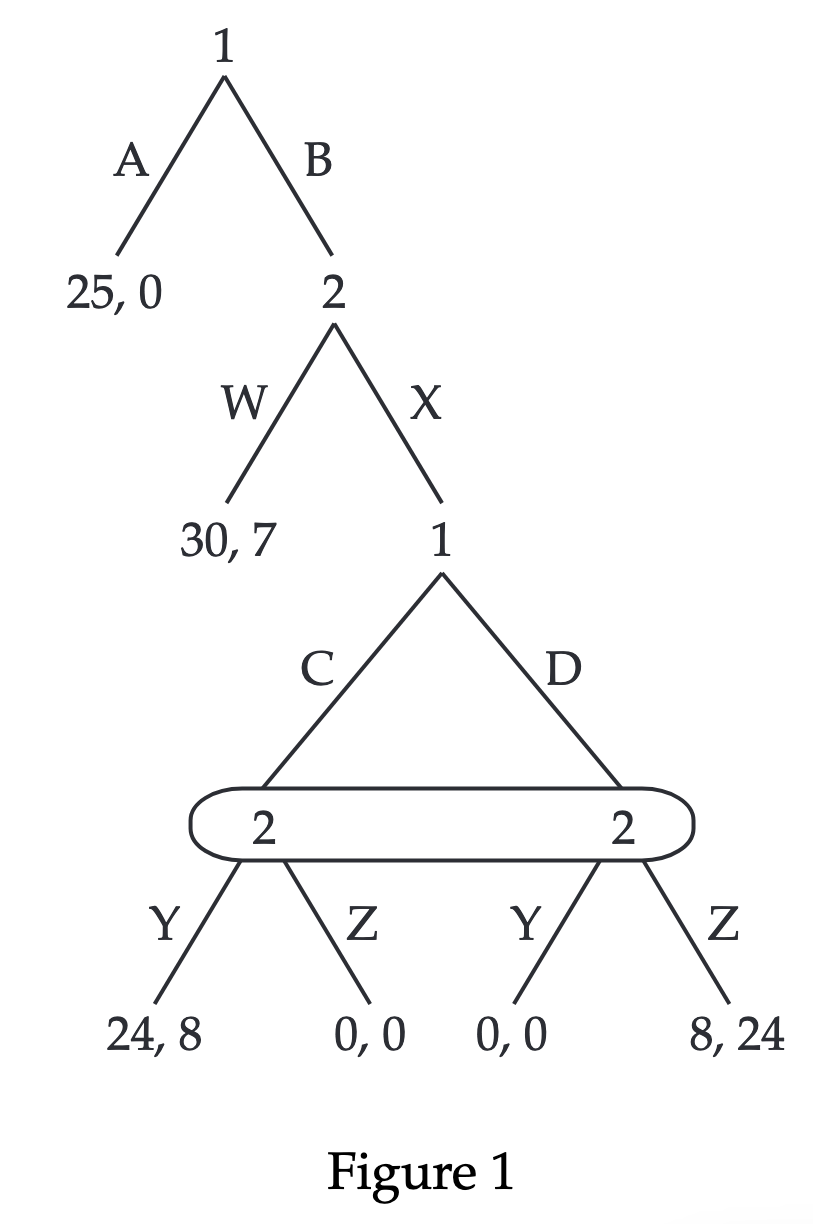
\includegraphics[width = 0.25\textwidth]{fig1.png}
  \end{center}
\section*{Problem 3. Sandholm PS3 \# 7}
  (i) Find all subgame perfect equilibria of the game in Figure 3 below when $z=3$.
  (ii) Determine the reduced normal form of this game when $z=3$.
  \begin{center}
    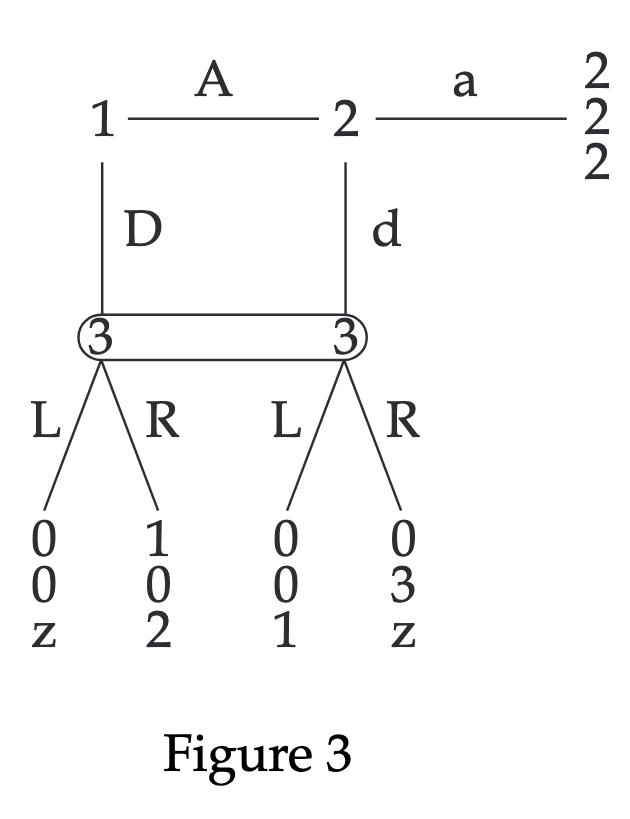
\includegraphics[width=0.25\textwidth]{fig3.png}
  \end{center}
\section*{Problem 4. Sandholm PS4 \# 1}
  Compute all sequential equilibria of the game in Figure 3 when $z=3$.
\section*{Problem 5. Sandholm PS4 \# 2}
  Compute all sequential equilibria of the game in Figure 3 when $z=2$.
\section*{Problem 6. Sandholm PS4 \# 3}
  For the game in Figure 4 below, specify an assessment (i.e., a strategy profile and a belief profile) with these three properties: (i) beliefs are Bayesian; (ii) no player has a profitable one-shot deviation at any information set; (iii) the assessment is not a weak sequential equilibrium.
  \begin{center}
    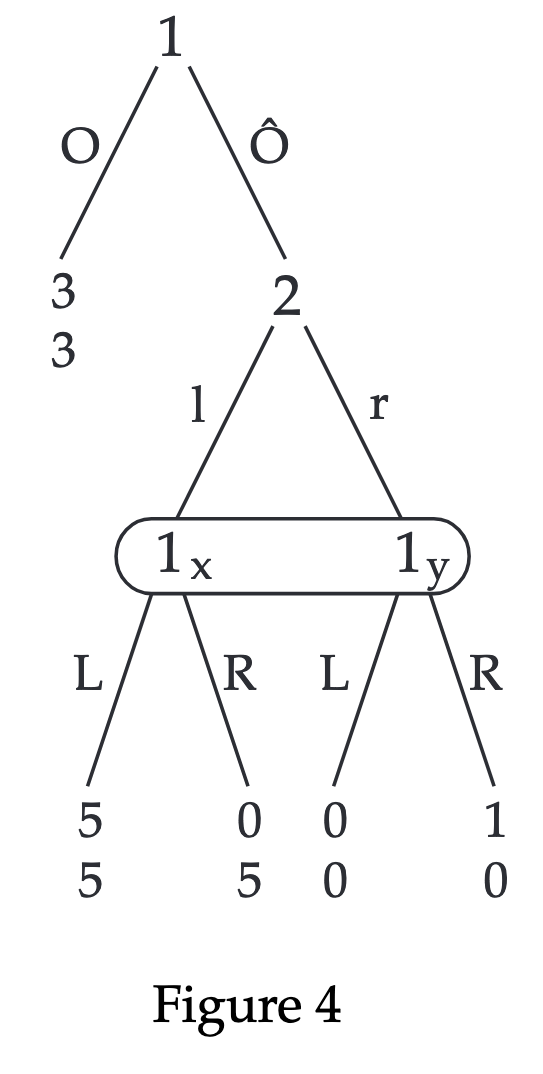
\includegraphics[width = 0.25\textwidth]{fig4.png}
  \end{center}
\end{document}
